\documentclass[conference]{IEEEtran}
\usepackage{cite}
\usepackage{amsmath,amssymb,amsfonts}
\usepackage{algorithmic}
\usepackage{graphicx}
\usepackage{textcomp}
\usepackage{xcolor}
\usepackage{fancyhdr}
\usepackage[hyphens]{url}

\def\BibTeX{{\rm B\kern-.05em{\sc i\kern-.025em b}\kern-.08em
    T\kern-.1667em\lower.7ex\hbox{E}\kern-.125emX}}

% Ensure letter paper
\pdfpagewidth=8.5in
\pdfpageheight=11in


%%%%%%%%%%%---SETME-----%%%%%%%%%%%%%
\newcommand{\iscasubmissionnumber}{NaN}
%%%%%%%%%%%%%%%%%%%%%%%%%%%%%%%%%%%%

\fancypagestyle{firstpage}{
}  


\pagenumbering{arabic}

%%%%%%%%%%%---SETME-----%%%%%%%%%%%%%
\title{CSE 240A Project Report: Branch Prediction} 
\author{Ke Wan, Xi Cai \\
Department of Computer Science \& Engineering \\
University of California San Diego

}
%%%%%%%%%%%%%%%%%%%%%%%%%%%%%%%%%%%%

\begin{document}
\maketitle
\thispagestyle{firstpage}
\pagestyle{plain}



%%%%%% -- PAPER CONTENT STARTS-- %%%%%%%%

\begin{abstract}

Branch prediction is very important to accelerate the speed of program and reduce stall time. This paper introduces three branch predictors, including G-Share branch predictor, Tournament branch predictor, and custom Perceptron branch predictor. 
This paper describes the structures of three branch predictors, the prediction and training method details, the implementation details, and experiment environment for developing and testing branch predictors. This paper uses six 
address traces to test misprediction rate of three branch predictors. The conclusion is that G-Share branch predictor and Tournament branch predictor have the similar performance. And custom Perceptron branch predictor performs 
the best among three predictors. It consumes the smallest memory space and beats the other two branch predictors in all six address traces. 

\end{abstract}

\section{introduction}
Branch instruction plays an important role on instruction sets. About 20\% of all computer instructions are branch instructions. However, branch instructions are
different from other kinds of instructions. There are multiple outcomes for a branch instruction. For example, for an \textbf{if-else} branch, there are two outcomes for this branch. 
If the value of the condition statement is true, then the program will execute the statements in the \textbf{if} code block. If not, the program will execute the statements
in the \textbf{else} code block. 

If we have an efficient branch predictor and can predict the outcome of branches correctly, then we can load the following instructions in advance to reduce stall time. 
This is the main advantage of branch predictor. But there are some disadvantages for branch predictors. Firstly, branch predictors will consume additional memory space and calculation resources, which will provide 
extra pressure for hardware. Secondly, it is risky to employ a branch predictor. We cannot make sure that a branch predictor can work well on every address trace. Fortunately, for most of the case, branch predictors 
provide more advantages than disadvantages. Now the state-of-the-art branch predictors achieve near perfect prediction accuracy on the vast majority of static branches. 

In this paper, we introduce three branch predictors, G-Share branch predictor, Tournament branch predictor, and custom Perceptron branch predictor. 
We discuss the structure, the design ideas, and the implementation details of these three branch predictor.

G-Share predictor is the most simple branch predictor in this paper. It fetched the lowest 13-bit Program Counter(PC) and Global History Address(GHA). Then we did an XOR calculation for these two variables
and map the result to Prediction History Table(PHT) to fetch the 2-bit prediction result. 

Tournament branch predictor is a hybrid predictor. It contains a local branch
predictor, a global branch predictor, and a choice predictor. Firstly, the Tournament branch predictor will fetch the lowest 10 bits of global history as the index of choice prediction. Then the branch predictor 
will determine which branch predictor should be used. If the branch predictor chooses to use the local predictor, then it will firstly fetch the lowest 9-bit PC as the index of Local History Table(LHT), then it 
will fetch the 10-bit Local History(LH) from LHT as the index of 2-bit local prediction result. If the branch predictor chooses the global predictor, then
it will firstly get the lowest 10 bits global address as the index of global prediction table. Then it will fetch the 2-bit prediction result from global PHT.

Our custom Perceptron branch predictor is based on Perceptron Predictor~\cite{nicepaper4}, which contains 16 weights per Perceptron to determine the prediction result. It contains a Table of Preceptron to store the perceptron weights for different local
history records and a register to store global history record. When the predictor encounters a branch, it will get the lowest 9 bits of PC address as the index of Perceptron Table. Then it will fetch the weights from the table and do
the prediction calculation using the formula $y_{out}=w_0+\sum_{i=1}^{n}{x_iw_i}$. If the value of $y_{out}$ is equal or greater than zero, then the branch predictor will predict it as TAKEN. Otherwise, the branch predictor will predict it as NOT-TAKEN. 

This paper also did experiments to test the prediction accuracy of three branch predictors on six address traces provided by instructors and made comparisons quantitatively. 
G-Share branch predictor achieves average accuracy of \textbf{94.41\%}. Tournament branch predictor achieves the average accuracy of \textbf{95.28\%}, a little better than G-Share predictor. 
The custom Perceptron branch predictor preforms the best among these three branch predictor. It has the average accuracy of \textbf{96.31\%}, and it beats the other two branch predictor in all six traces. 


\section{responsibility of each member}
This project is finished by two members, Ke Wan and Xi Cai. Ke Wan mainly contributes to design, develop, and test Tournament 
and custom Perceptron branch predictor. Xi Cai mainly contributes to develop G-share branch predictor and verified the 
correctness of our implementations. We cooperated to write project report. 

\section{background and motivation}
Branch instruction plays an important role on instruction sets. About 20\% of all computer instructions are branch instructions. However, branch instructions are
different from other kinds of instructions. There are multiple outcomes for a branch instruction. Predicting the outcome of branches correctly is important to accelerate the speed of instruction execution and reduce the stall time. 
If we have an excellent branch predictor, then we will fetch the next instructions correctly in most of the time with less stall time. However, if we have a terrible branch predictor, then
we will find that the program will fetch wrong instructions in most of the time, which increases the execution time of the program. Therefore, having an excellent branch predictor can help us
accelerate the speed of the program further. This is our motivation to develop branch predictor. 

During lectures, Prof. Zhao showed us two simple but efficient branch predictors. One is G-Share branch predictor, and 
the other is Tournament branch predictor. We implemented both of them in this paper. Moreover, Prof. Zhao encourages us to go further in this path. Therefore, we made research and implemented custom 
Perceptron branch predictor with a better performance. 

\section{design ideas}
The main task of a branch predictor is to predict whether or not the branch will be taken given the Program Counter(PC). Usually, a branch predictor maintains a global/local history table and a prediction table
in order to help predict the outcome of a branch. In this paper, we provide three branch predictors. They are G-Share branch predictor, Tournament branch predictor, and Custom Perceptron branch predictor. 
In this section, for every branch predictor, we will describe the prediction and training design ideas. Note that for every prediction method, the input parameter is PC, and the output value is TAKEN or NOT-TAKEN. For 
training method, the input parameters are PC and outcome. There is no output for training method. 
\subsection{G-Share branch predictor}
\begin{center}
  \textbf{Prediction}
\end{center}

G-Share branch predictor is one of the most simple but efficient branch predictors, which uses PC and global history table to make predictions. In this project, we use G-Share 13 predictor, which means that 
we get the lowest 13-bit PC and global history table to make hash calculation in order to get the index for prediction table.
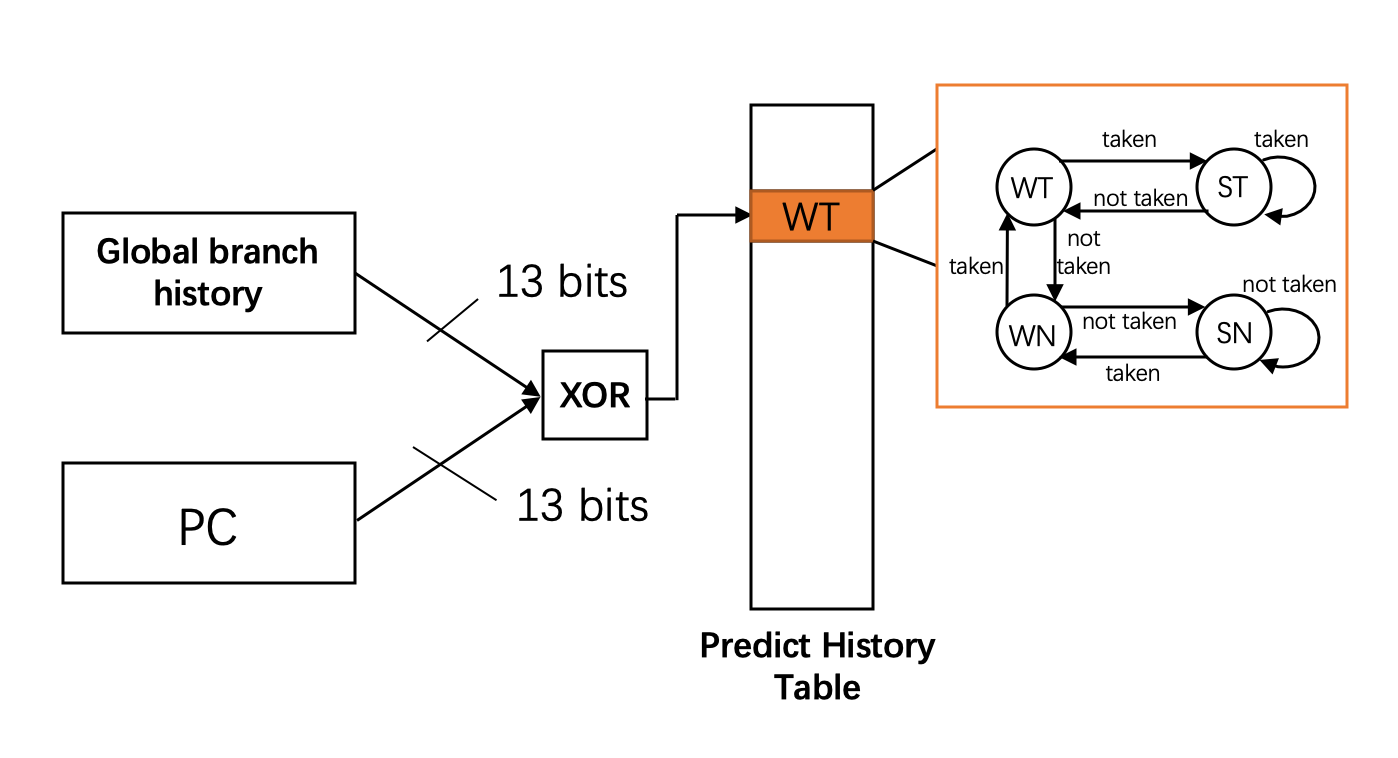
\includegraphics[width=\linewidth]{g-share.png}
\begin{center}
  {\small Figure 1. G-Share predictor}
\end{center}

As Figure 1 indicated, we get the lowest 13-bit PC and global history table and make a XOR calculation. The result is the index for prediction table.
The finite-state machine for prediction result is also contained in Figure 1. G-Share branch predictor employs 2-bit 
history-based branch prediction. The values in prediction table are 2-bit unsigned integers, 
where 0 is strongly not taken(SN), 1 is weakly not taken(WN), 2 is weakly taken(WT), and 3 is strongly taken(ST). We can pick the prediction result from this table. 
Take the entry in Figure 1 for example, the value of this prediction is WT, which means that the predictor will predict Weakly Taken for this PC.

\begin{center}
  \textbf{Training}
\end{center}
The training process for G-Share predictor includes two steps. The first one is to update picked value in prediction table, and the second one is to update global history table. 
For picked value in prediction table, the branch predictor follows the finite-state machine in Figure 1 to update the prediction result for the selected entry given the PC and outcome. 
For global history table, the predictor will shift the bits in global history register to left by 1, and put the outcome to the least significant bit of the global history register. 

\subsection{Tournament branch predictor}
Tournament branch predictor is a hybrid predictor. Why is it called "hybrid"? Because it contains two branch predictor. One is global branch predictor, and the other one is local branch predictor. 
The architecture of Tournament branch predictor is shown in Figure 2. 
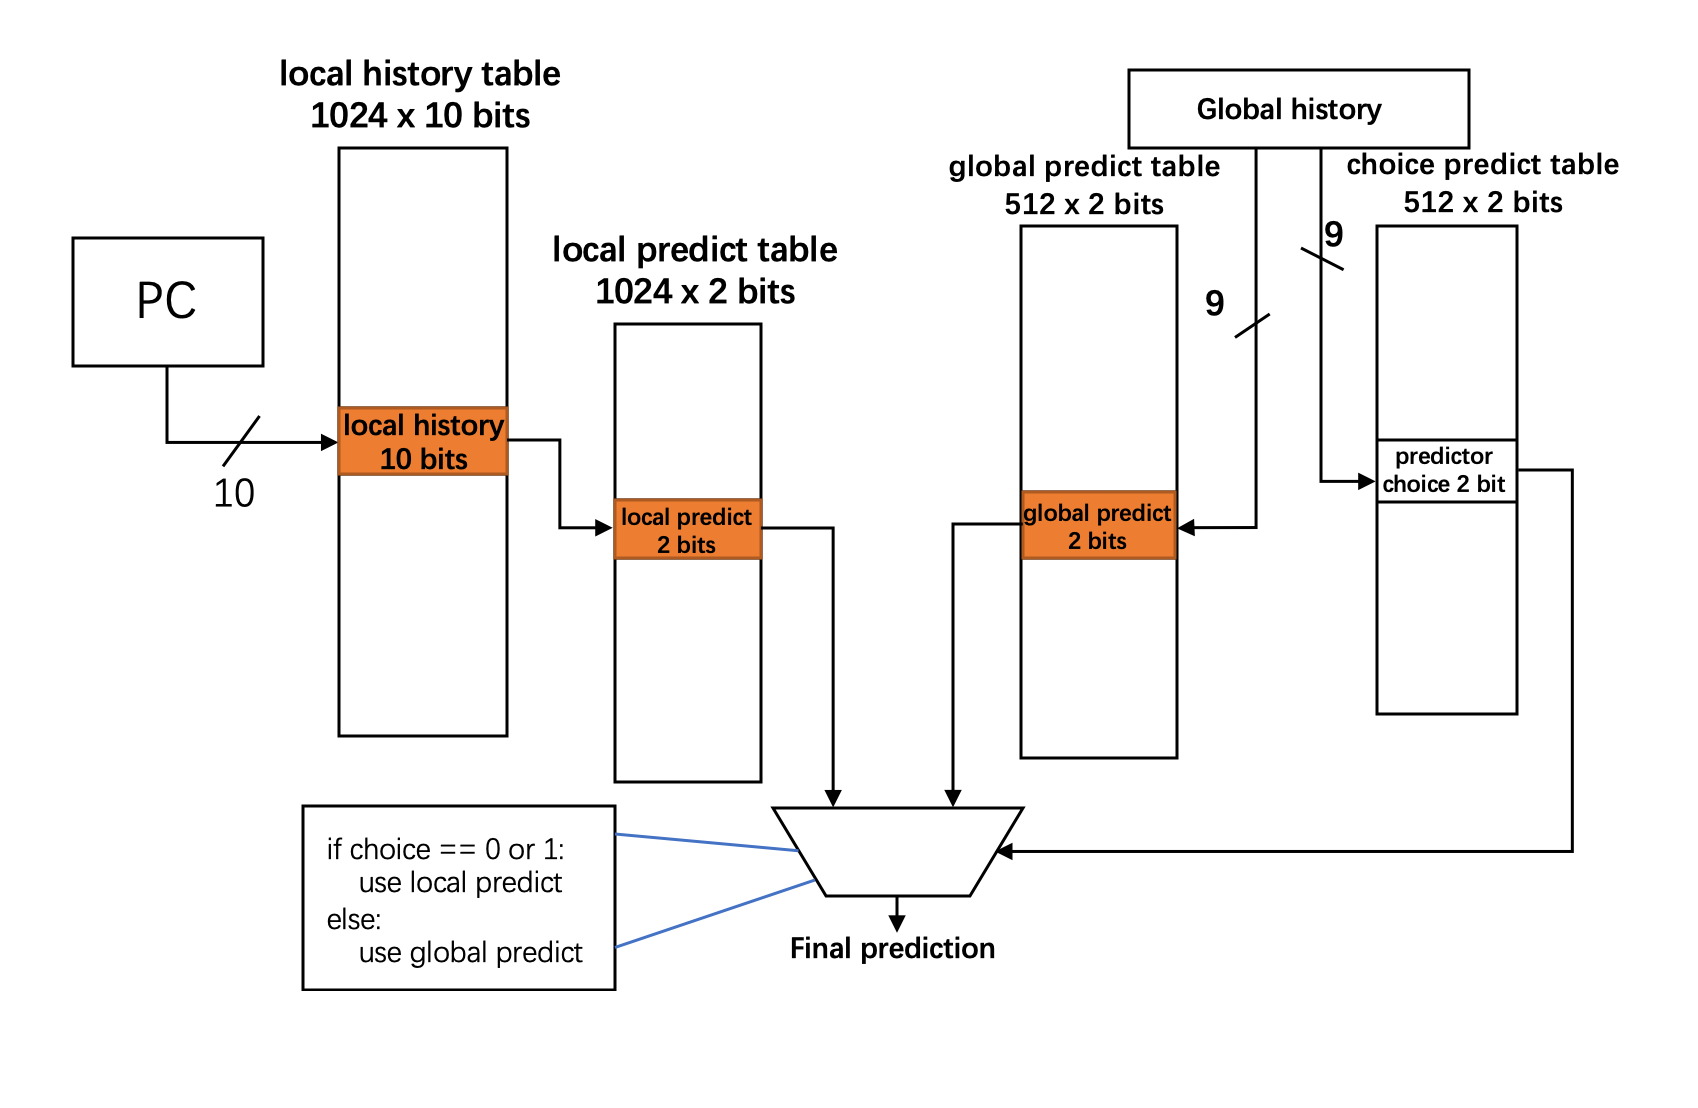
\includegraphics[width=\linewidth]{Tournament.png}
\begin{center}
  {\small Figure 2. Tournament branch predictor}
\end{center}
In this paper, we use Tournament 9:10:10, which means that we assign 9 bits for global history, 10 bits for local history, and 10 bits for PC. We also referred Alpha 21264 Microprocessor Architecture ~\cite{nicepaper5}.  

\begin{center}
  \textbf{Prediction}
\end{center}
While making a prediction, the first step is to determine which branch predictor should we use. We firstly pick the lowest 9-bit global history as the index of choice table. Then we pick the value of choice table as our predictor choice. 
The values in choice table employ 2-bit history-based prediction, and it contains four statuses: strongly local, weakly local, weakly global, and strongly global. After deciding which branch predictor we use, we then make predictions for branches. 

If we decide to use local branch predictor, we firstly pick the lowest 10-bit PC address as the index of local history table. 
We get the local history for this PC address. Then we pick the lowest 10-bit local history as the index of local prediction table. The values in local prediction table is the local prediction, which are 2-bit unsigned integers. 
Local prediction has the same set of status as G-Share predictor, containing SN, WN, WT, and ST. 

If we decide to use global predictor, we firstly pick the lowest 9-bit global history as the index of global prediction table. Then we pick the prediction result from global prediction table. 
The values in the global prediction table are 2-bit prediction results, which have the same set of statuses as local predictor. 

After getting the prediction result, we will have finished prediction with Tournament branch predictor. 

\begin{center}
  \textbf{Training}
\end{center}
The training process for Tournament branch predictor contains four steps. The first step is to make predictions using local and global branch predictors using PC. The second step is to update the 
picked Choice Table value following the finite state machine shown in Figure 3 based on prediction results of local predictor and global predictor.
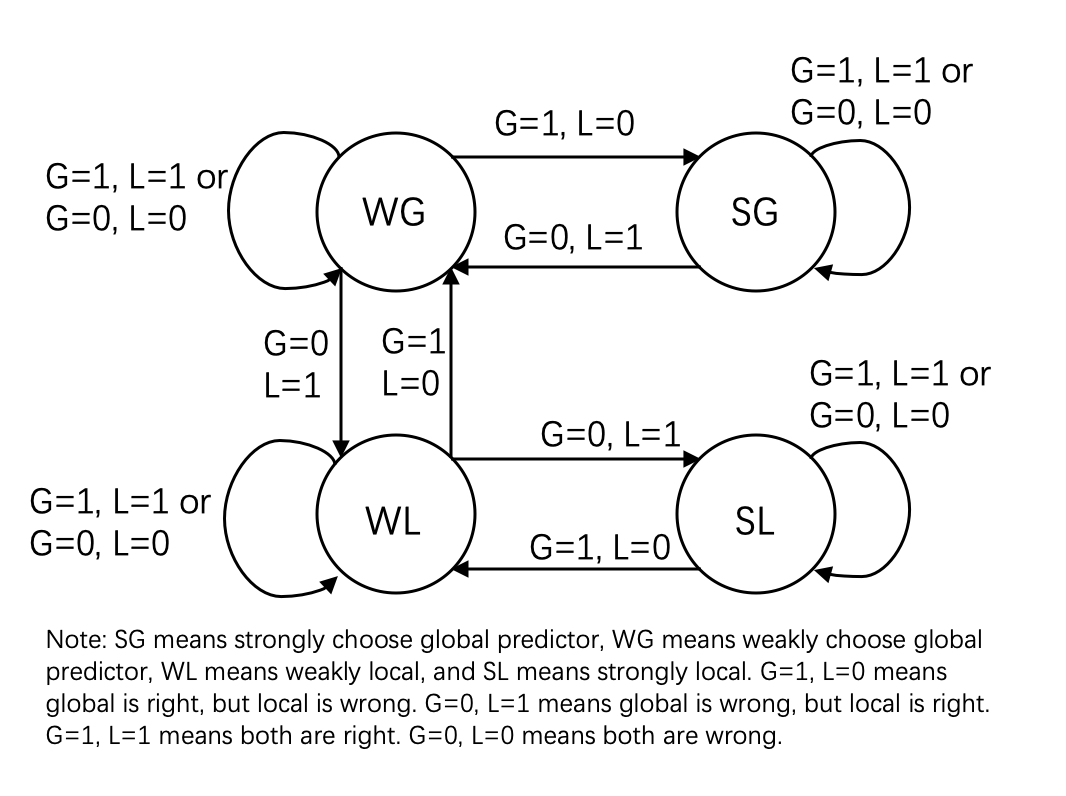
\includegraphics[width=\linewidth]{choice-machine.png}
\begin{center}
  {\small Figure 3. Choice value finite state machine}
\end{center}
The third step is to update local predictor and global predictor following 2-bit branch prediction rules. The last step is to update global history table and the picked value in local history table. The 
update process is the same as G-Share branch predictor. 

\subsection{Custom Perceptron branch predictor}
Our custom Preceptron branch predictor employs the idea from Dynamic Branch Prediction with Perceptrons paper~\cite{nicepaper4}, which is a micro neural network architecture. The architecture of this branch predictor is shown in Figure 4.
There are two storage structures in this branch predictor. The first one is Perceptron Table, which contains weights for different branches. Since we get the lowest 9 bits from PC, there will be 512 entries for Perceptron Table. 
Every Perceptron contains 16 weights including a biased variable. Every weight is a 8-bit integer, ranging from -128 to 127. Therefore, the size of Perceptron Table is $512*16*8 = 64k  bits$, which satisfies the project requirement. 
The second one is global history table, which consists of fifteen 8-bit integers to record the latest 15 outcomes. The remaining integer is the biased variable, and it doesn't consume memory space. 
The size of global history table is $15*8 = 120  bits$, which also satisfies the project requirement.

\begin{center}
  \textbf{Prediction}
\end{center}
For making a prediction, the first step is to get the lowest 9-bit PC as the index of Perceptron Table. Then the predictor will use this index to get the weights from Perceptron Table and make a inner product between Global History Table and the weights.
The inner product result is stored in variable Y. Then the predictor will compare the value of Y with zero. If the value of Y is equal to or greater than zero, then the predictor will predict it as Taken. Otherwise, the predictor will predict it as 
Not Taken.

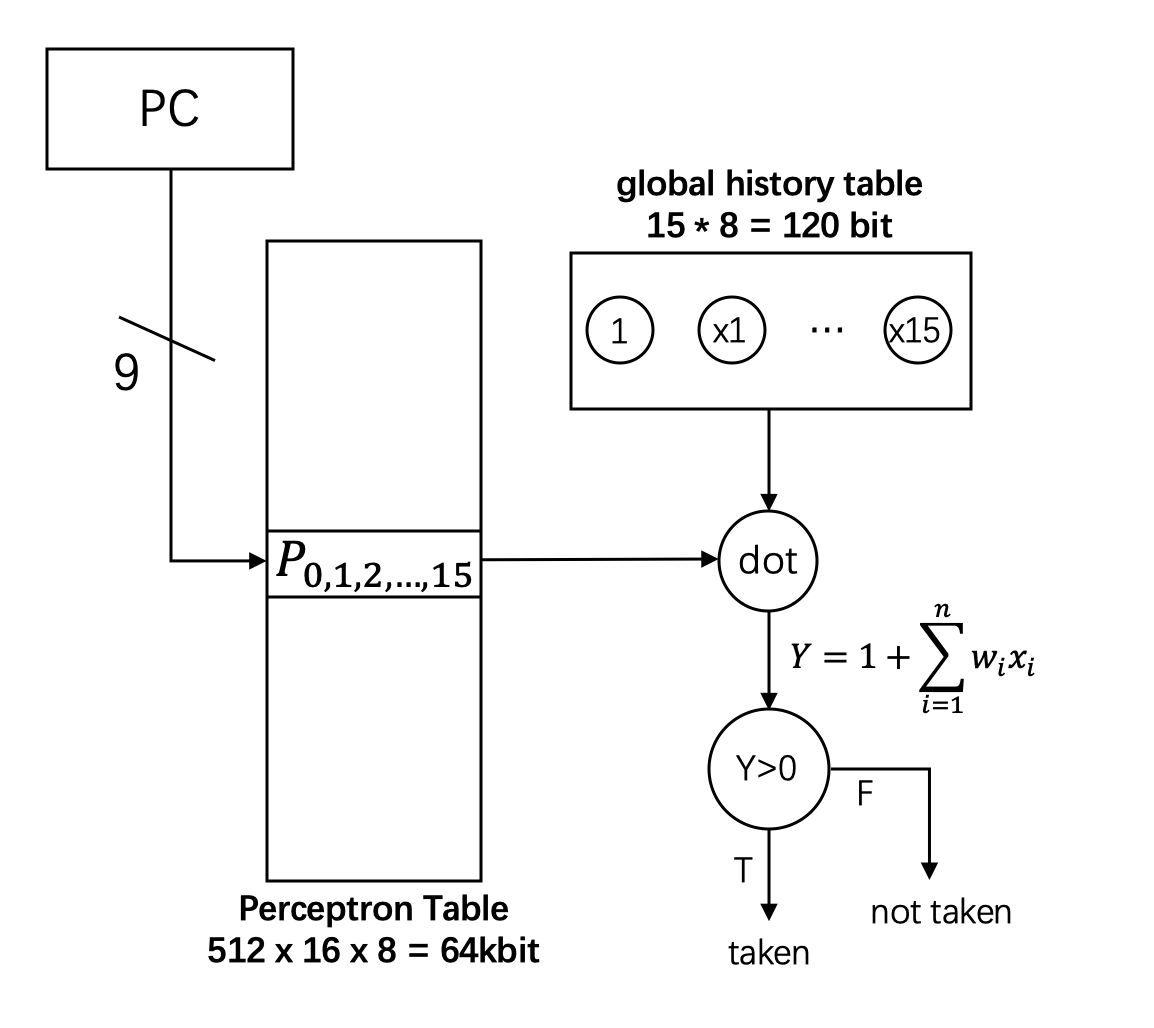
\includegraphics[width=\linewidth]{perceptron.png}
\begin{center}
  {\small Figure 4. Custom Preceptron branch predictor}
\end{center}

\begin{center}
  \textbf{Training}
\end{center}
The training process of custom Preceptron branch predictor has two steps. The first one is to update selected weights, and the second step is to update global history table. For updaing selected weights, we followed section 3.3 and section 6 in Dynamic Branch Prediction with Perceptrons paper~\cite{nicepaper4}. 
For updating global history table, we follow the same path as G-Share predictor. 

\section{implementation}
\subsection{G-Share predictor}
For initial function, we set global history table register as zero. We also assign the prediction table with memory space. For the values in prediction table, the initial value should be Weakly Not Taken(WN). For training and prediction function, we just follow the Design Idea to implement them. 
\subsection{Tournament branch predictor}
For initial function, we set global history table register as zero and assign memory space for local history table, local prediction table, global prediction table, and choice prediction table.
For values in local and global prediction table, the initial value should be WN. And for values in choice prediction table, the initial value should be Weakly Global(WG). The initial values in local history table
 are all set to zero. For training and prediction method, we follow the Design Ideas to implement them. 
\subsection{Custom Preceptron branch predictor}
For initial function, we assign memory space for Perceptron Table and global history table. The weights in Perceptron Table are all set to zero. The values in global history table are all set to zero. For training and prediction function, we just follow the Design Idea to implement them.
\section{experiment setup and results}
We employ Docker Image provided by instructors as our experiment environment. We develop our project in our local environment and run the code in the Docker container. We ran all three branch predictors on six address traces. And
the experiment result is shown in Table 1. G-Share means G-Share 13 branch predictor, Tournament means Tournament 9:10:10 branch predictor, and Custom means custom Perceptron branch predictor. 
Note that the numbers in the table are misprediction rate. 

\begin{scriptsize}
\begin{table}[h!]
  \centering
  \caption{misprediction rate of three branch predictors}
  \label{table:formatting}
  \begin{tabular}{|l|l|l|l|}
    \hline
    \textbf{Trace} & \textbf{G-Share} & \textbf{Tournament} & \textbf{Custom}\\
    % \hline
    \hline
    fp\_1 & 0.825 & 0.991 & 0.824\\
    \hline
    fp\_2 & 1.678 & 3.246 & 1.302\\
    \hline
    int\_1 & 13.839 & 12.622 & 10.370\\
    \hline
    int\_2 & 0.420 & 0.426 & 0.346\\
    \hline
    mm\_1 & 6.696 & 2.581 & 2.161\\
    \hline
    mm\_2 & 10.138 & 8.483 & 7.163\\
    \hline
    average & 5.6 & 4.72 & 3.69\\
    \hline
  \end{tabular}
\end{table}
\end{scriptsize}

\section{conclusion}
From Table 1, we can conclude that the performance of G-Share branch predictor and Tournament branch predictor are both great. They can both achieve average misprediction rate less than 6. But 
Tournament branch predictor has a lower average misprediction rate than G-Share branch predictor. 
G-Share branch predictor beats Tournament branch predictor on fp\_1, fp\_2, and int\_2. But Tournament branch predictor beats G-Share branch predictor on int\_1, mm\_1. and mm\_2. 

The best performer among these branch predictor is custom Perceptron branch predictor. It has the lowest misprediction rate. And it beats both G-Share branch predictor and Tournament branch predictor in all
six address traces. Moreover, it only consumes 64k + 120 bits memory space, but both G-Share branch predictor and Tournament branch predictor consume more than 100k bits memory space. Therefore, we can conclude that our 
custom Perceptron branch predictor has the best performance. 

We discussed the reason for this result. For Tournament branch predictor, we observe that the average misprediction rate is lower than G-Share branch predictor. 
The reason is that Tournament branch predictor has two branch predictors. One is local branch predictor, and the other is global branch predictor. Tournament branch predictor can decide which branch predictor to use 
based on the input PC and choice history. This is advantageous for the Tournament branch predictor to get a better choice. However, G-Share branch predictor only has one branch predictor. 
If the address trace relys more on local history than on global history, then the G-Share branch predictor will perform badly and it cannot do better because it doesn't have a local branch predictor. 
But sometimes, the choice predictor cannot predict which predictor performs better correctly, and sometimes neither of these two predictors can predict correctly. Therefore, for some address traces, the performace of Tournament 
branch predictor doesn't perform better than G-Share branch predictor. And the overall performance of Tournament branch predictor is better than G-Share branch predictor. 

For custom Perceptron branch predictor, the secret comes from neural network structure. Neural network can simulate both linear and non-linear functions. It has a strong learning capability. Given suffcient dataset, the neural network can do training and store the learning results in weights.
The weights are helpful for neural network to do predictions. Therefore, with the same dataset, neural network can learn faster than 2-bit branch prediction. And this is the reason why custom Perceptron branch predictor performs the best. 
Additionally, custom Perceptron branch predictor does not need to store all local history and the past prediction results. Rather, it only needs to store weights and global history in memory. Therefore, it uses
less memory space than G-Share branch predictor and Tournament branch predictor. 
%%%%%%% -- PAPER CONTENT ENDS -- %%%%%%%%


%%%%%%%%% -- BIB STYLE AND FILE -- %%%%%%%%
\bibliographystyle{IEEEtranS}
\bibliography{refs}
%%%%%%%%%%%%%%%%%%%%%%%%%%%%%%%%%%%%

\end{document}

